\section{The Vanishing Gradient Problem}

% -----------------------------------------------------------------------------
\begin{frame}\frametitle{\secname}
	\begin{center}
		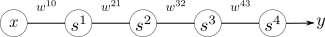
\includegraphics[width=10cm]{img/simple_arch}
	\end{center}
    forward pass
    \begin{align}
    y\;\;&=\;\;
    f(h^{4})\\
    \;\;&=\;\;
    f\big(w^{43} \cdot f(h^{3})\big)\\
    \;\;&=\;\;
    f\Big(w^{43} f\big(w^{32} \cdot f(h^{2})\big)\Big)\\
    \;\;&=\;\;
    f\bigg(w^{43} f\Big(w^{32} \cdot f\big(w^{21} \cdot f(h^{1})\big)\Big)\bigg)\\
    \;\;&=\;\;
    f\bigg(w^{43} f\Big(w^{32} \cdot f\big(w^{21} \cdot f(w^{10} \cdot x)\big)\Big)\bigg)
    \end{align}
\end{frame}

% -----------------------------------------------------------------------------
\begin{frame}\frametitle{\secname}
	\begin{center}
		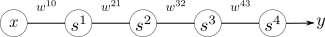
\includegraphics[width=10cm]{img/simple_arch}
	\end{center}
    backward pass:
    \begin{align}
     \frac{\partial y}{\partial w^{10}}
     \;\;&\stackrel{\mathclap{
    \substack{\text{chain}\\ \text{rule}}}
    }{=}\;\;
    \frac{\partial y}{\partial h^{1}}
    \cdot \frac{\partial h^1}{\partial w^{10}}\\
    \;\;&=\;\;
    \frac{\partial y}{\partial h^{2}}
    \cdot \frac{\partial h^{2}}{\partial h^{1}}
    \cdot \frac{\partial h^1}{\partial w^{10}}\\
    \;\;&=\;\;
    \frac{\partial y}{\partial h^{3}}
    \cdot \frac{\partial h^{3}}{\partial h^{2}}
    \cdot \frac{\partial h^{2}}{\partial h^{1}}
    \cdot \frac{\partial h^1}{\partial w^{10}}\\
    \;\;&=\;\;
    \frac{\partial y}{\partial h^{4}}
    \cdot \frac{\partial h^{4}}{\partial h^{3}}
    \cdot \frac{\partial h^{3}}{\partial h^{2}}
    \cdot \frac{\partial h^{2}}{\partial h^{1}}
    \cdot \frac{\partial h^1}{\partial w^{10}}\\
    \;\;&=\;\;
    =f'(h^{4}) w^{43} \cdot f'(h^{3}) w^{32} \cdot f'(h^{2}) w^{21} \cdot f'(h^{1}) w^{10}
    \end{align}
\end{frame}


